\chapter{Dispositivos Fotovoltaicos\label{cha:DispositivosFotovoltaicos}}

Este capítulo es un breve resumen de los aspectos más importantes
sobre el funcionamiento de las células y módulos fotovoltaicos. El
lector interesado puede acudir a las referencias \cite{Lorenzo2006c,Green1995,Wenham.Green.ea2000}
para ampliar estos contenidos y a la referencia \cite{LopezAraujo1986}
para estudiar la física de los dispositivos electrónicos.


\section{Funcionamiento de una célula solar}

La corriente de una célula solar es un balance entre la fotocorriente
y la corriente de oscuridad que, a su vez, depende de la tensión aplicada
en los terminales del dispositivo. Esta relación se representa en
la figura \ref{fig:CurvaIVCelula}. Cuando la tensión aplicada es
nula (la célula está cortocircuitada) la corriente se debe exclusivamente
a la fotocorriente. El valor de la corriente permanece casi constante
hasta las cercanías del valor de tensión en el que el diodo comienza
a conducir. A partir de este punto, la corriente disminuye abruptamente
hasta alcanzar un valor nulo (célula en circuito abierto) en el punto
donde la fotocorriente y la corriente de oscuridad quedan compensadas. 


%
\begin{figure}
\begin{centering}
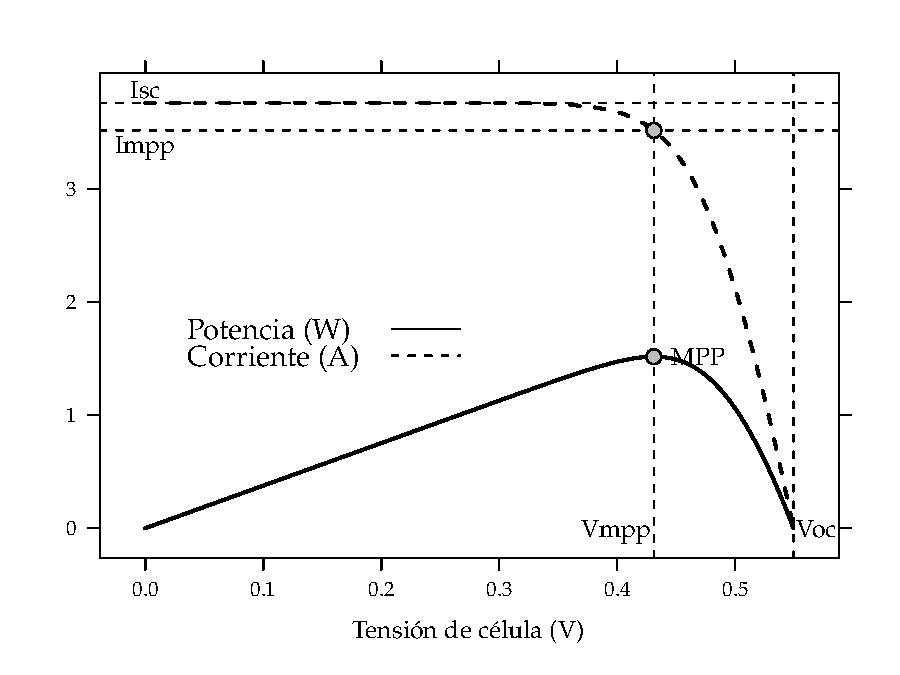
\includegraphics[scale=0.75]{../figs/CurvaIV_Ta20_G800}
\end{centering}

\caption[Curvas corriente-tensión y potencia-tensión de una célula solar]{Curvas corriente-tensión (línea discontinua) y potencia-tensión (línea
continua) de una célula solar.\label{fig:CurvaIVCelula}}

\end{figure}



Los dos puntos extremos de cortocircuito y circuito abierto quedan
definidos con dos parámetros, la corriente de cortocircuito, $I_{sc}$,
y la tensión de circuito abierto, $V_{oc}$. Estos dos parámetros
suelen estar disponibles en la información asociada a una célula.
En función de ellos se puede escribir la ecuación \ref{eq:EcuacionCelulaInicial},
que describe la curva característica de una célula:

\begin{equation}
I=I_{sc}\cdot\left[1-\exp\left(\frac{e\cdot(V_{oc}-V)}{m\cdot k\cdot T_{c}}\right)\right]\label{eq:EcuacionCelulaInicial}\end{equation}
\nomenclature[Isc]{$I_{sc}$}{Corriente de cortocircuito de una célula}\nomenclature[Voc]{$V_{oc}$}{Tensión de circuito abierto de una célula}


\subsection{Punto de máxima potencia}

Superpuesta a la curva corriente-tensión, la figura \ref{fig:CurvaIVCelula}
incluye la relación entre la potencia y la tensión. Es evidente la
presencia de un máximo que adquiere el nombre de punto de máxima potencia
(\emph{MPP, maximum power point }en sus siglas inglesas). La localización
de este punto viene definida por la condición $\frac{\mathrm{d}P}{\mathrm{d}V}=0$.
La potencia entregada por la célula en este punto será la considerada
como potencia nominal, $P_{mpp}=I_{mpp}\cdot V_{mpp}$.\nomenclature[Impp]{$I_{mpp}$}{Corriente en el punto de máxima potencia de una célula}\nomenclature[Vmpp]{$V_{mpp}$}{Tensión en el punto de máxima potencia de una célula}\nomenclature[Pmpp]{$P_{mpp}$}{Potencia en el punto de máxima potencia de una célula}
Las unidades de esta potencia son vatios pico (Wp), reflejando la
idea de potencia máxima alcanzable.

Dado que la célula funciona en corriente continua, su potencia es
$P=V\cdot I$ y por tanto:

\begin{eqnarray}
\frac{\mathrm{d}(I\cdot V)}{\mathrm{d}V} & = & V\cdot\frac{\mathrm{d}I}{\mathrm{d}V}+I\cdot\frac{\mathrm{d}V}{\mathrm{d}V}\nonumber \\
\mathrm{d}P & = & V\cdot\mathrm{d}I+I\cdot\mathrm{d}V\end{eqnarray}


Antes de este punto, $\frac{\mathrm{d}P}{\mathrm{d}V}>0$ o, de
forma equivalente, $\frac{\mathrm{d}I}{\mathrm{d}V}>-\frac{I}{V}$.
Entre este punto y el circuito abierto $\frac{\mathrm{d}P}{\mathrm{d}V}<0$
o, de forma equivalente, $\frac{\mathrm{d}I}{\mathrm{d}V}<-\frac{I}{V}$.
En el punto de máxima potencia se cumplirá:\begin{equation}
\frac{\mathrm{d}I}{\mathrm{d}V}=-\frac{I_{mpp}}{V_{mpp}}\label{eq:MPP_derivada}\end{equation}



\subsection{Factor de forma y Eficiencia}

El área encerrada por el rectángulo definido por el producto $I_{mpp}\cdot V_{mpp}$
es, cómo es observable en la figura \ref{fig:CurvaIVCelula}, inferior
a la representada por el producto $I_{sc}\cdot V_{oc}$. La relación
entre estas dos superficies se cuantifica con el factor de forma:

\begin{equation}
FF=\frac{I_{mpp}\cdot V_{mpp}}{I_{sc}\cdot V_{oc}}\label{eq:FactorForma}\end{equation}
\nomenclature[FF]{FF}{Factor de forma}

El factor de forma es tanto más cercano a la unidad cuánto mas acentuado
sea el codo localizado en el punto de máxima potencia. Su valor, normalmente
comprendido entre $0.7$ y $0.8$, varía poco de unas células a otros.
Conociendo los valores de $I_{sc}$ y $V_{oc}$ es posible calcular
la potencia en el punto de máxima potencia, dado que $P_{mpp}=FF\cdot I_{sc}\cdot V_{oc}$.

Por otra parte, la calidad de una célula se puede cuantificar con
la eficiencia de conversión según la ecuación \ref{eq:EficienciaCelula}

\begin{equation}
\eta=\frac{I_{mpp}\cdot V_{mpp}}{P_{L}}\label{eq:EficienciaCelula}\end{equation}
\nomenclature[eta]{$\eta$}{Eficiencia de una célula}donde $P_{L}$
representa la potencia luminosa que incide en la célula. Como es evidente
de la ecuación \ref{eq:EficienciaCelula}, este valor de eficiencia
se corresponde al caso en el que el acoplamiento entre la carga y
la célula permite a ésta trabajar en el punto de máxima potencia.
Las células industriales de silicio suelen ofrecer eficiencias comprendidas
entre el 13\% y el 17\%.


\subsection{Condiciones estándares de medida}
\label{sec:STC}

Se definen unas condiciones de funcionamiento, denominadas condiciones
estándar de medida (\emph{STC, standard test conditions} en sus siglas
inglesas), válidas para caracterizar una célula o un módulo en un
laboratorio de medida. Esta condiciones vienen determinadas por:

\begin{itemize}
\item Irradiancia: $G_{stc}=\SI{1000}{\watt\per\meter\squared}$
\nomenclature[Gstc]{$G_{stc}$}{Irradiancia incidente en condiciones
  estandar de medida}
\nomenclature[STC]{STC}{Condiciones estándar de medida}
con incidencia normal.
\item Temperatura de célula: $T_{c}^{*}=\SI{25}{\celsius}$
\nomenclature[Tc]{$T_{c}$}{Temperatura de célula}
\nomenclature[Tcstc]{$T_{c}^{*}$}{Temperatura de célula en condiciones estandar de medida}.
\item Masa de aire: $AM=1.5$
\end{itemize}

Es de uso común añadir un asterisco como superíndice para denotar
aquellos parámetros medidos en estas condiciones. Frecuentemente los
fabricantes informan de los valores de las tensiones $V_{oc}^{*}$
y $V_{mpp}^{*}$ y las corrientes $I_{sc}^{*}$ y $I_{mpp}^{*}$.
A partir de estos valores es posible referir a estas condiciones la
potencia, $P_{mpp}^{*}=I_{mpp}^{*}\cdot V_{mpp}^{*}$, el factor de
forma, $FF^{*}=\frac{P_{mpp}^{*}}{I_{sc}^{*}\cdot V_{oc}^{*}}$
y la eficiencia:

\begin{equation}
\eta^{*}=\frac{I_{mpp}^{*}\cdot V_{mpp}^{*}}{A\cdot G_{stc}}
\label{eq:EficienciaCelula_STC}
\end{equation}


\subsection{Circuito equivalente de una célula solar}

Para analizar el comportamiento de una célula en un circuito es conveniente
emplear modelos equivalentes alternativos a la ecuación \ref{eq:EcuacionCelulaInicial}.
La corriente fotogenerada puede ser modelada con un generador de corriente
mientras que la corriente de oscuridad puede ser representada con
un diodo, tal y como se recoge en la figura \ref{fig:M=0000F3deloCelula}.
En esta figura se incluyen una resistencia serie y una resistencia
paralelo para efectos no incluidos en la ecuación \ref{eq:EcuacionCelulaInicial}
pero apreciables en las células reales. 

%
\begin{figure}
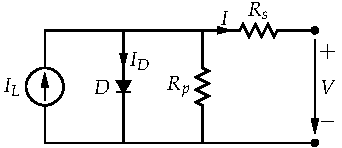
\includegraphics{../figs/ModeloElectricoCelulaSolar}\caption{Modelo eléctrico de una célula solar.\label{fig:M=0000F3deloCelula}}

\end{figure}


La resistencia serie representa la resistencia debida a los contactos
metálicos con el semiconductor, a las capas semiconductoras y a la
malla de metalización. Esta resistencia reduce principalmente el factor
de forma y, en menor medida, la corriente de cortocircuito. Es interesante
comprobar que, una vez conocidos los valores de los cuatro parámetros
eléctricos de la célula ($I_{sc}$, $V_{oc}$, $I_{mpp}$, $V_{mpp}$),
es posible obtener el valor de $R_{s}$\nomenclature[Rs]{$R_{s}$}{Resistencia serie de una célula}
a partir de la ecuación \ref{eq:RsDatosFabricante} a partir de la
información que el fabricante suministra sobre las corrientes y tensiones
del dispositivo: \begin{equation}
R_{s}^{*}=\frac{V_{oc}^{*}-V_{mpp}^{*}+m\cdot
  V_{t}\cdot\ln(1-\frac{I_{mpp}^{*}}{I_{sc}^{*}})}{I_{mpp}^{*}}
\label{eq:RsDatosFabricante}
\end{equation}
\nomenclature[m]{m}{Factor de idealidad del módelo del diodo}\nomenclature[Vt]{$V_{t}$}{Potencial térmico}

La resistencia paralelo representa las fugas de corriente en los bordes
de célula, los posibles cortocircuitos metálicos y la recombinación
favorecida en las fronteras de grano del cristal. Esta resistencia
reduce el factor de forma y la tensión de circuito abierto. En general,
toma valores suficientemente altos como para que su influencia en
el funcionamiento global sea baja, y de ahí que frecuentemente se
desprecie su contribución. Además, considerando que el valor de la
exponencial es notablemente superior a 1 en todas las condiciones
de operación y que la corriente de cortocircuito es equivalente a
la corriente fotogenerada, se obtiene la ecuación que emplearemos
como curva característica de la célula solar: \begin{equation}
I=I_{sc}[1-\exp(\frac{V-V_{oc}+I\cdot R_{s}}{m\cdot V_{t}})]\label{eq:EcuacionCelulaFinal}\end{equation}



\section{El módulo fotovoltaico}

Las características eléctricas de una célula no son suficientes para
alimentar las cargas convencionales. Es necesario realizar agrupaciones
en serie y paralelo para entregar tensión y corriente adecuadas. Un
módulo fotovoltaico es una asociación de células a las que protege
físicamente de la intemperie y aisla eléctricamente del exterior,
dando rigidez mecánica al conjunto. 

Existen multitud de módulos diferentes, tanto por su configuración
eléctrica como por sus características estructurales y estéticas.
En general, la asociación de células es encapsulada en dos capas de
EVA (etileno-vinilo-acetato), entre una lámina frontal de vidrio y
una capa posterior de un polímero termoplástico (frecuentemente se
emplea el tedlar) u otra lámina de cristal cuando se desea obtener
módulos con algún grado de transparencia. Muy frecuentemente este
conjunto es enmarcado en una estructura de aluminio anodizado con
el objetivo de aumentar la resistencia mecánica del conjunto y facilitar
el anclaje del módulo a las estructuras de soporte.

El vidrio frontal debe tener y mantener una alta transmisividad en
la banda espectral en la que trabajan las células solares. Además,
debe tener buena resistencia al impacto y a la abrasión. Su superficie
debe ser de forma que combine un buen comportamiento antireflexivo
con la ausencia de bordes o desniveles que faciliten la acumulación
de suciedad o dificulten la limpieza de ésta mediante la acción combinada
del viento y la lluvia. Frecuentemente se emplea vidrio templado con
bajo contenido en hierro con algún tipo de tratamiento antireflexivo.

El encapsulante a base de EVA, combinado con un tratamiento en vacío
y las capas frontal y posterior, evita la entrada de humedad en el
módulo, señalada como la causa principal de la degradación a largo
plazo de módulos fotovoltaicos. Además, esta combinación permite obtener
altos niveles de aislamiento eléctrico \cite{Wenham.Green.ea2000}. 

Una configuración eléctrica muy común hasta hace unos años empleaba
36 células en serie para obtener módulos con potencias comprendidas
en el rango $\SIrange[range-phrase=-]{50}{100}{\Wp}$ con tensiones
en MPP cercanas a los $\SI{15}{\volt}$ en funcionamiento. Estos módulos
eran particularmente adecuados para su acoplamiento con baterías de
tensión nominal $\SI{12}{\volt}$ en los sistemas de electrificación
rural. Con el protagonismo abrumador de los sistemas fotovoltaicos
de conexión a red, esta configuración ha perdido importancia. Ahora
son frecuentes los módulos de potencia superior a los $\SI{200}{\Wp}$
y tensiones en el rango $\SIrange[range-phrase=-]{30}{50}{\volt}$.

Para los módulos compuestos por células de silicio cristalino es de
aplicación la norma internacional IEC 61215 {}``\emph{Crystalline
Silicon Terrestrial Photovoltaic (PV) Modules - Design Qualification
and Type Approval}''. Esta norma internacional recoge los requisitos
de diseño y construcción de módulos fotovoltaicos terrestres apropiados
para su operación en períodos prolongados de tiempo bajo los efectos
climáticos. Asimismo, esta norma detalla un procedimiento de pruebas
a los que se debe someter el módulo que desee contar con la certificación
asociada a esta normativa.


\subsection{Influencia de la temperatura y la radiación}

En un módulo compuesto por $N_{cs}$ células en serie y $N_{cp}$
ramas en paralelo, y suponiendo que las células que lo forman son
idénticas, la tensión del módulo es $V_{m}=N_{cs}\cdot V_{c}$ y la
corriente del módulo es $I_{m}=N_{cp}\cdot I_{c}$, siendo $V_{c}$
e $I_{c}$ la tensión y la corriente de una célula, respectivamente,
la curva característica de un módulo puede calcularse de forma aproximada
con:

\begin{equation}
I_{m}=I_{sc}\cdot\left(1-exp\left(\frac{V_{m}-V_{oc}+I_{m}\cdot
      R_{s}}{V_{t}}\right)\right)
\end{equation}


Como aproximación, se supone que la corriente de cortocircuito depende
exclusivamente y de forma lineal de la irradiancia:
\begin{equation}
I_{sc}=G_{ef}\cdot\frac{I_{sc}^{*}}{G_{stc}}
\end{equation}
y la tensión de circuito abierto depende exclusivamente de la temperatura
de \emph{célula}, y decrece linealmente con ella:
\begin{equation}
V_{oc}(T_{c})=V_{oc}^{*}+(T_{c}-T_{c}^{*})\cdot\frac{dV_{oc}}{dT_{c}}
\end{equation}
Si no hay información específica por parte del
fabricante, para células de silicio cristalino es habitual emplear el valor:
\begin{equation}
dV_{oc}/dT_{c} = \SI{-2.3}{\milli\volt\per\celsius}
\label{eq:VocTemperatura}
\end{equation}
\nomenclature[Tc]{$T_{c}$}{Temperatura de funcionamiento de una
  célula}
\nomenclature[dVoc]{$dV_{oc}/dT_{c}$}{Variación de la tensión de circuito abierto con la temperatura de célula}

En estas dos ecuaciones se hace referencia a las condiciones estándar
de medida. En estas condiciones, la temperatura de \emph{célula} es
de $\SI{25}{\celsius}$. Sin embargo, la temperatura de operación
de la célula depende de la temperatura ambiente y la irradiancia incidente.
La ecuación \ref{eq:TONC} expresa una aproximación aceptable del
comportamiento térmico de un módulo:\begin{equation}
T_{c}=T_{a}+G_{ef}\cdot\frac{NOCT-20}{800}\label{eq:TONC}\end{equation}
\nomenclature[TONC]{TONC}{Temperatura nominal operacional de célula}

En esta ecuación se emplea el concepto de temperatura de operación
nominal de célula (NOCT o TONC) definida como aquella que alcanza
una \emph{célula} cuando su \emph{módulo} trabaja en las siguientes
condiciones:
\needspace{5\onelineskip}
\begin{itemize}
\item Irradiancia: $G=\SI{800}{\watt\per\meter\squared}$
\item Espectro: el correspondiente a $AM=1.5$\nomenclature[AM]{AM}{Masa de aire}.
\item Incidencia normal
\item Temperatura \emph{ambiente}: $T_{a}=\SI{20}{\celsius}$.
\item Velocidad de viento: $v_{v}=\SI{1}{\meter\per\second}$\nomenclature[vv]{$v_{v}$}{Velocidad de viento}.
\end{itemize}
El valor de la TONC suele estar incluido dentro de la información
que el fabricante recoge en su ficha técnica. No obstante, un valor
de $\SI{47}{\celsius}$ es aceptable para un amplio rango de módulos
fotovoltaicos de silicio cristalino.

El efecto de la temperatura en la curva característica queda recogido
en la figura \ref{fig:EfectoTemperaturaUNED} y el efecto de la irradiancia
en la figura \ref{fig:EfectoIrradianciaUNED}. Es fácil comprobar
que la corriente y la potencia aumentan con el nivel de irradiancia
incidente, y la tensión y la potencia disminuyen con la temperatura
ambiente.


%
\begin{figure}
\begin{centering}
\subfloat[Curva I-V.]{\begin{centering}
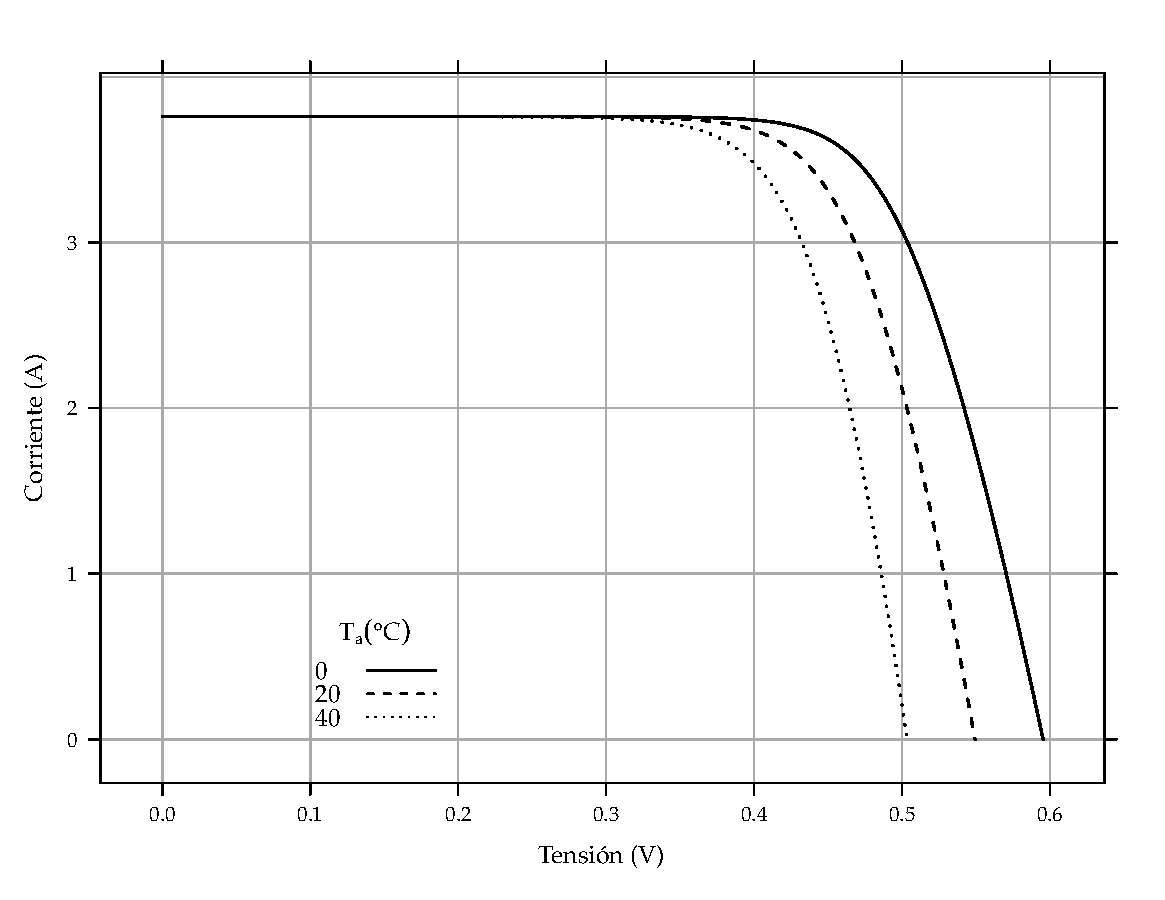
\includegraphics[scale=0.7]{../figs/CurvaIV_G800}
\par\end{centering}

}
\par\end{centering}

\begin{centering}
\subfloat[Curva P-V.]{\begin{centering}
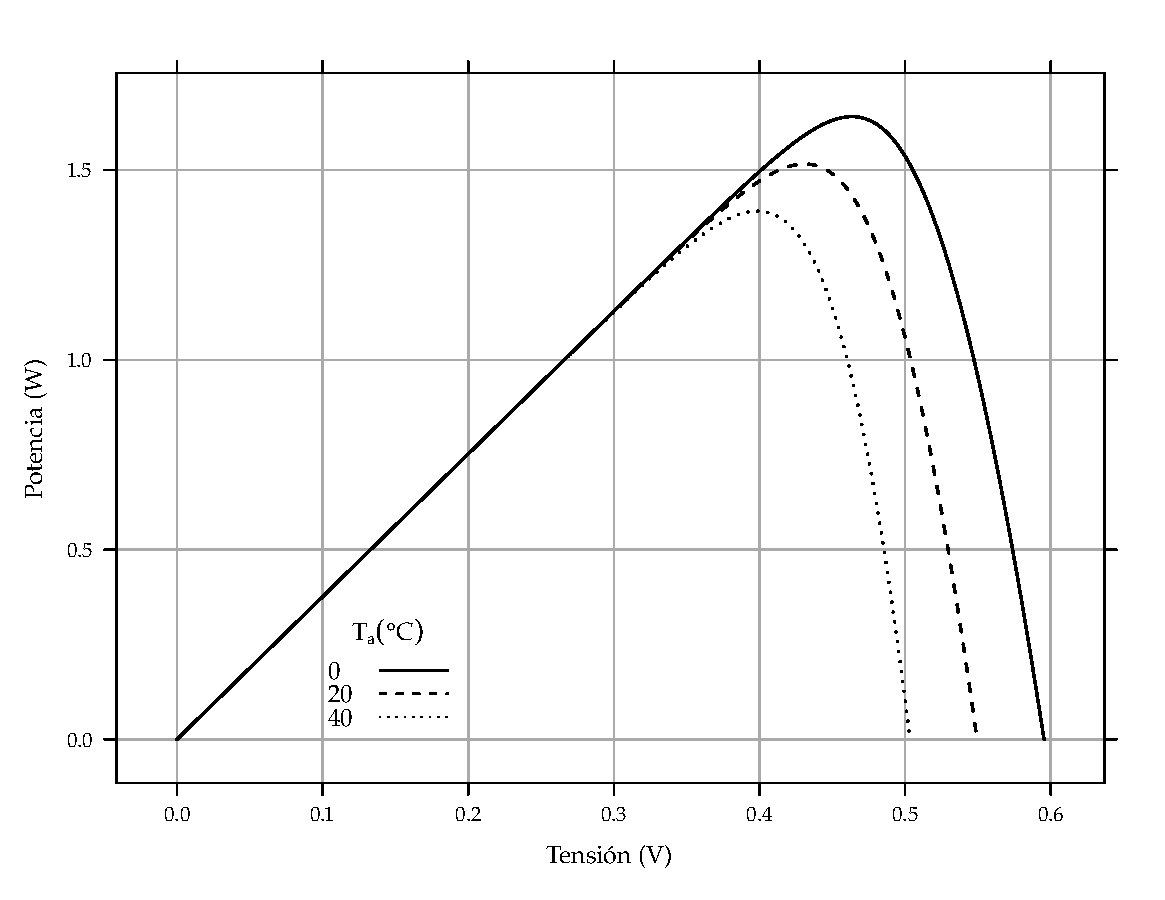
\includegraphics[scale=0.7]{../figs/CurvaPV_G800}
\par\end{centering}



}
\end{centering}

\caption{Efecto de la temperatura en la curva característica de una célula
solar ($G=\SI{800}{\watt\per\meter\squared}$).\label{fig:EfectoTemperaturaUNED}}

\end{figure}




%
\begin{figure}
\begin{centering}
\subfloat[Curva I-V.]{\begin{centering}
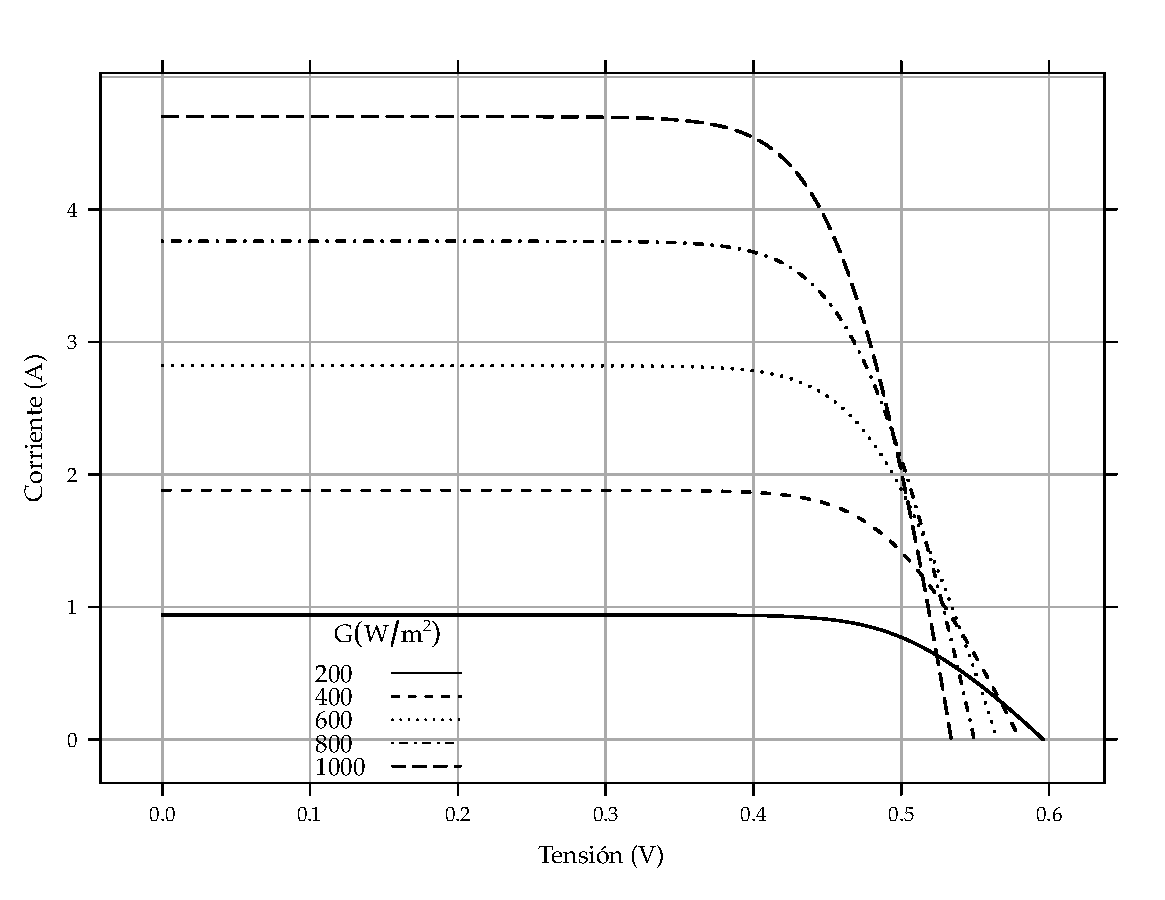
\includegraphics[scale=0.7]{../figs/CurvaIV_Ta20}
\par\end{centering}

}
\par\end{centering}

\begin{centering}
\subfloat[Curva P-V.]{\begin{centering}
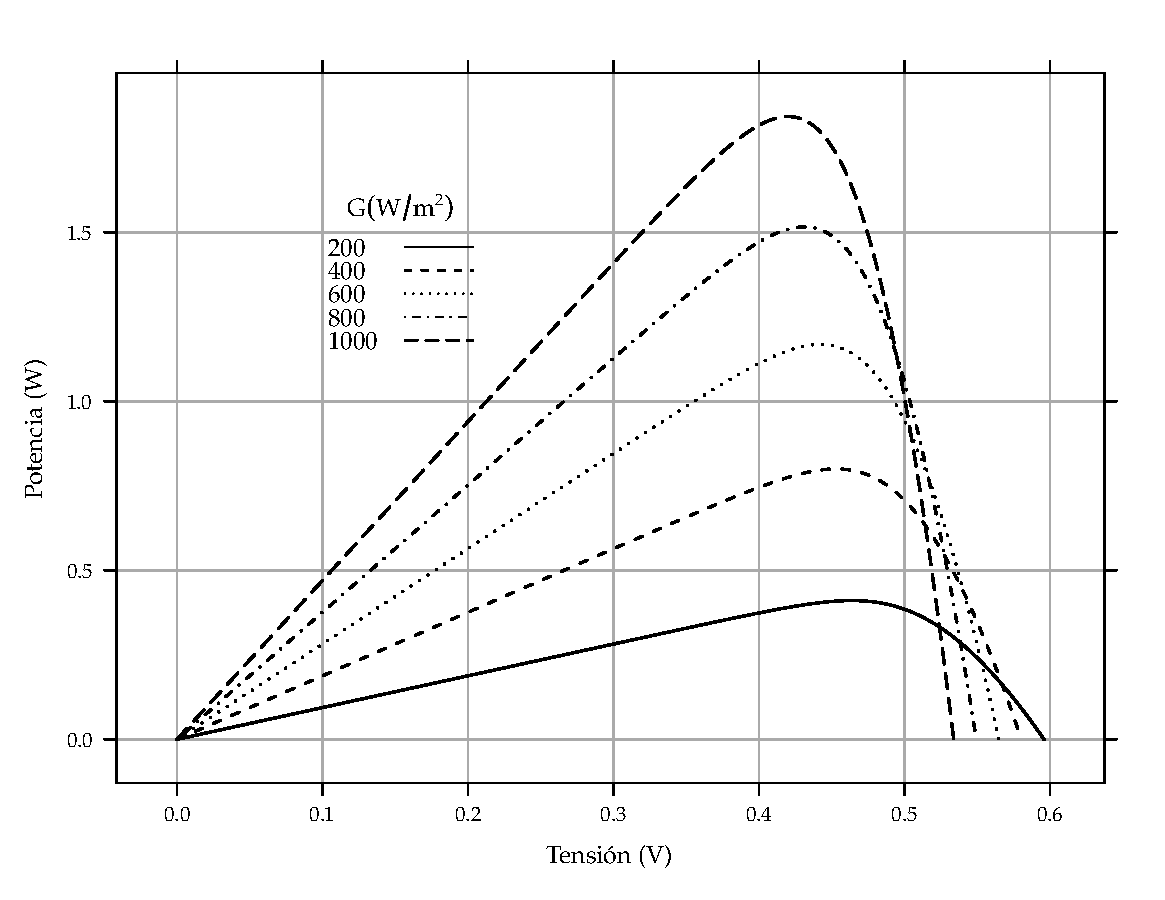
\includegraphics[scale=0.7]{../figs/CurvaPV_Ta20}
\par\end{centering}



}
\end{centering}

\caption{Efecto de la irradiancia en la curva característica de una célula
solar ($T_a=\SI{20}{\celsius}$).\label{fig:EfectoIrradianciaUNED}}

\end{figure}



%%% Local Variables:
%%% mode: LaTex
%%% TeX-master: "ESF.tex"
%%% End: 